\chapter{Bluetooth Mesh}
\label{ch:Ble_mesh}

% https://www.bluetooth.com/learn-about-bluetooth/bluetooth-technology/topology-options/
Per soddisfare al meglio le esigenze di connettività wireless di applicazioni così diversificate, la tecnologia Bluetooth supporta più topologie. Dalle semplici connessioni \textit{point-to-point} ottimizzata per lo streaming audio adottando la tecnologia Bluetooth classic e per il trasferimento dati (Fitness Tracker, Health monitor, etc) attraverso l'uso della tecnologia BLE, alle comunicazioni \textit{Broadcast} ottimizzate per la condivisione di informazioni localizzate (come punti d'interesse, indicazioni stradali, tacking di articoli, etc) e alle reti \textit{Mesh} introdotte per la creazione di reti di dispositivi su larga scala ed ideali per sistemi di controllo, monitoraggio e automazioni in cui decine (ma anche centinaia o migliaia) di dispositivi devono comunicare in modo affidabile e sicuro tra loro.\\

\noindent Bluetooth Low Energy inizialmente supportava solo due tipologie di comunicazione: \textit{one-to-one} (Connection-oriented communication) in cui due dispositivi devono connettersi tra loro per scambiarsi dati utente e \textit{one-to-many} (Connection-less communication) in cui un dispositivo si trova nello stato di Advertising e provvede ad inviare in broadcast i propri dati pubblici a qualsiasi dispositivo adiacente interessato, senza dover prima stabilire una connessione.\\
Una cosa che mancava alla tecnologia BLE era la capacità di supportare una comunicazione \textit{many-to-many} in cui dispositivi potessero scambiarsi messaggi e inoltrarli ad altri nodi all'interno di una rete. Tale esigenza ha portato al rilascio dello standard Bluetooth Mesh da parte di Bluetooth SIG nel luglio del 2017.\\
% Immagine Topologie di comunicazione BLE
% https://embeddedcentric.com/lesson-2-ble-profiles-services-characteristics-device-roles-and-network-topology/

\noindent L'introduzione della rete mesh ha portato a due principali benefici:
\begin{itemize}
    \item \textit{Extended range}: indica che le informazioni possono essere trasmesse da un nodo all'altro finché non giungono al destinatario. Tale politica consente ad una rete di estendere il suo raggio d'azione e ampliare la portata di ogni singolo messaggio.
    
    \item \textit{Self-healing capabilities}: indica che non esiste un singolo punto di fallimento. Se un nodo della rete subisce un guasto, gli altri possono comunque continuare a partecipare e inviarsi i messaggi l'un l'altro.
\end{itemize}

\section{Architettura}
% https://www.bluetooth.com/learn-about-bluetooth/bluetooth-technology/topology-options/le-mesh/mesh-glossary/
% https://www.bluetooth.com/blog/the-fundamental-concepts-of-bluetooth-mesh-networking-part-1/      ---- [part-1, part-2]
% https://www.novelbits.io/bluetooth-mesh-tutorial-part-1                                           ---- [part-1, part-2]
Bluetooth Mesh è eseguito al di sopra dello standard BLE e opera attraverso gli stati Advertising e Scanning per l'invio e la ricezione dei messaggi tra i nodi all'interno di una rete mesh. Ciò significa che i dispositivi che fanno parte di una rete mesh Bluetooth non si connettono tra loro ma piuttosto scambiano informazioni tra loro utilizzando pacchetti advertising; tipologia di pacchetti ricevuta da tutti i dispositivi nello stato di Scanning.
La figura \ref{fig:ble_mesh_architecture} delinea lo stack BLE Mesh e di seguito sono definite le funzionalità di ciascun livello \cite{bluetooth2019b, afaneh2018intro}.
\begin{figure}[!ht]
    \centering
    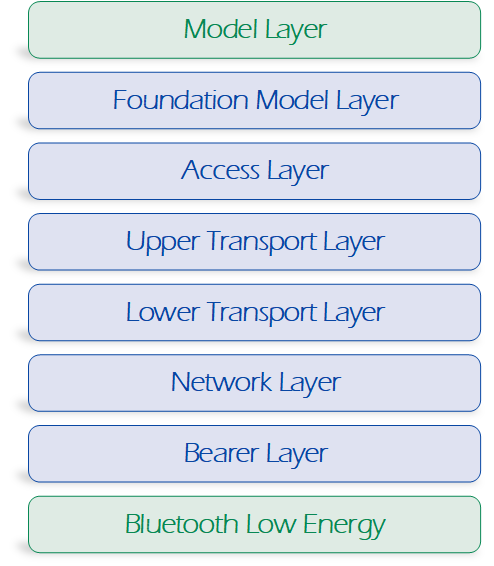
\includegraphics[width = 0.9\textwidth]{images/Layer BLE Mesh.png}
    \caption{Architettura Bluetooth Mesh}
    \label{fig:ble_mesh_architecture}
\end{figure}
\begin{itemize}
    \item il \textit{Model layer} definisce i modelli utilizzati per standardizzare il funzionamento di tipici scenari utente. Nello specifico definisce comportamenti, messaggi, stati e associazioni tra stati. Esempi tipici di modelli riguardano l'illuminazione ed i sensori.
    
    \item il \textit{Foundation Model layer} definisce gli stati, i messaggi e i modelli richiesti per configurare e gestire una rete mesh.
    
    \item l'\textit{Access layer} definisce come i livelli al di sopra di esso possono utilizzare l'upper transort layer, definendo la struttura dei dati, definendo e gestendo la cifratura e decodifica di tali dati (eseguito nell'upper transort layer). In più controlla se i dati in entrata rispettano la network e l'application key prima di inoltrarli al livello superiore.
    
    \item l'\textit{Upper Transort layer} si occupa della cifratura, decodifica e convalida dei dati provenienti dal livello applicazione e della riservatezza dei messaggi appartenenti al access layer. Definisce inoltre il modo in cui i messaggi di controllo (Heartbeat, Friednship, etc.) sono utilizzati e trasportati tra i nodi.
    
    \item il \textit{Lower Transort layer} definisce il modo in cui i messaggi del livello superiore (upper transort layer) vengono segmentati al fine di rispettare i limiti imposti sulle dimensioni dei pacchetti. In caso di messaggi segmentati, provenienti dal livello sottostante, prevede di riassemblarli (in modo da ricostituire il pacchetto originale) prima di trasmetterli al livello superiore.
    
    \item il \textit{Network layer} definisce come i messaggi del livello di trasporto vengono indirizzati verso uno o più elementi. Definisce il formato dei pacchetti a livello di rete (network PDU) che consente alle Lower Transport PDU di essere trasportate dal livello sottostante (Bearer layer). Decide se inoltrare o meno un messaggio, accettarlo per ulteriori elaborazioni o rifiutarlo. Inoltre, si occupa delle cifratura e dell'autenticazione dei messaggi in arrivo e in uscita.
    
    \item il \textit{Bearer layer} definisce un'astrazione della specifica BLE sottostante per i livelli superiori, difatti definisce come differenti tipi di pacchetti (Protocol Data Unit) devono essere gestiti e trasportati tra i nodi dell'intera rete mesh. Lo standard definisce due tipi Bearer\footnote{stack protocollare usato per trasportare dati tra endpoint per conto di un altro stack protocollare posizionato sopra di esso. In questo caso consente di trasportare diverse tipologie di PDU all'interno di una rete mesh}: Advertising bearer e GATT bearer. \\
    Quando si usa l'Advertising bearer, un pacchetto mesh deve essere inviato come Advertising Data all'interno della BLE advertising PDU e si utilizzano gli stati advertising e scanning durante la comunicazione.\\
    GATT bearer è stato introdotto per consentire ai dispositivi che non supportano gli Advertising bearer di interagire comunque con i nodi coinvolti in una rete mesh. Prevede l'utilizzato del protocollo Proxy per consentire la trasmissione e la ricezione di PDU tra i dispositivi attraverso una connessione GATT. Ciò è possibile attraverso il proxy node.

    \item Bluetooth Mesh per poter essere eseguito sui dispositivi richiede l'intero stack \textit{Bluetooth Low Energy}. Come anticipato in precedenza, opera negli stati di advertising e di scanning, in più supporta attraverso un nodo speciale, proxy node, anche la modalità Connected e le operazione GATT che consentono ad un nodo che supporta lo standard Bluetooth Mesh di interagire con i nodi appartenenti ad una rete mesh.
\end{itemize}

\subsection{Bluetooth Mesh Concepts}
% https://docs.espressif.com/projects/esp-idf/en/latest/api-guides/esp-ble-mesh/ble-mesh-terminology.html
Lo standard Bluetooth Mesh, anche se eseguito al disopra dello stack BLE, prevede l'impiego di ulteriori concetti finora non appartenenti ad uno standard Bluetooth. Tra cui l'utilizzo del paradigma Publish-Subscribe, l'utilizzo di apposite chiavi di sicurezza per la cifratura dei dati e concetti come quello di elementi e indirizzamento, per citarne alcuni. 
Tali concetti verranno affrontati di seguito.

\subsubsection{Network}
\label{subsub:network}
Una mesh Bluetooth è costituita da dispositivi che cooperano tra di loro e condividono delle risorse, come ad esempio: 
l'\textit{indirizzo di rete} usato per identificare il mittente e il destinatario di un messaggio; % Section 3.4.2
le \textit{chiavi} di \textit{rete} (NetKeys) e di \textit{applicazione} (AppKeys) usate per crittografare e autenticare un messaggio rispettivamente in merito al network layer e access layer.\\ % Section 3.8.6.3 e Section 3.8.6.2
Una rete può essere costituita da una o più sottoreti. Una sottorete racchiude un gruppo di nodi che per comunicare tra loro a livello di rete adottano la medesima network key. Un nodo può essere a conoscenza di una o più Netkeys, il che gli consente di appartenere a più sottoreti.\\
Una rete mesh Bluetooth può essere costituita al massimo da 32767 nodi e la massima distanza che un messaggio può percorrere, espressa in termini di hop, all'interno della rete è di 127 hop.

\subsubsection{Nodi}
\label{subsub:nodi}
Un \textit{nodo} è un dispositivo che si è unito ad una rete mesh Bluetooth. Un dispositivo, prima di entrare a far parte di una tale rete è identificato con il termine \textit{unprovisioned device}. Nel momento in cui entra a farvi parte, a seguito di un processo di \textit{provisioning} che consente di autenticare il dispositivo e comunicargli informazioni di base necessarie per la comunicazione con gli altri nodi appartenenti ad essa, viene identificato con il termine \textit{nodo}. Solo nel momento in cui assume il ruolo di nodo, il dispositivo è in grado di inviare, ricevere o inoltrare i messaggi appartenenti alla rete e può opzionalmente far parte anche di una o più sottoreti.\\
Un nodo all'interno della rete può assumere diversi ruoli in base alle features supportate e abilitate. I speciali quattro ruoli definibili (descritti nella sezione \ref{subsub:features}) sono i seguenti: \textit{Relay Node}, \textit{Proxy Node}, \textit{Friend Node} e \textit{Low Power Node}. \\
La procedura di provisioning (discussa in \ref{sec:provisioning}) coinvolge un nodo esterno chiamato Provisioner il cui compito è proprio quello di aggiungere un dispositivo ad una rete mesh.

\subsubsection{Elementi}
\label{subsub:elementi}
% un'entità indirizzabile all'interno di un dispositivo
Un nodo può essere costituito da più parti che possono essere controllate in modo indipendente. Ogni singola entità indirizzabile in modo univoco presente all'interno di un nodo è identificata come \textit{elemento}. Ogni nodo è costituito da almeno un elemento, denominato primary element. Gli altri elementi che costituiscono il nodo sono indicati o come elementi addizionali o come secondary element. Ogni elemento, sia esso primary sia secondary, contiene uno o più modelli e nel caso in cui sono contenuti più modelli, essi non devono essere uguali.\\
L'elemento primary è indirizzabile usando l'indirizzo univoco assegnato al nodo durante il processo di provisioning, mentre gli eventuali elementi addizionali sono raggiungibili utilizzando indirizzi successivi. Attraverso questi indirizzi univoci è possibile identificare all'interno di un nodo, quale elemento sta trasmettendo o ricevendo messaggi.\\
Ad esempio, un lampadario può contenere più lampadine che possono essere accese o spente in modo indipendente, ogni singola lampadina costituisce un elemento del nodo lampadario.

\subsubsection{Stati}
\label{subsub:stati}
Lo \textit{stato} è un valore che rappresenta una condizione di un elemento. Un elemento che espone uno stato è definito \textit{server}, mentre un elemento che accede ad uno stato è definito \textit{client}. Il più semplice esempio di server è un Generic OnOff Server in cui lo stato può essere `on' oppure `off', mentre un Generic OnOff Client è in in grado di gestire gli stati di un Generic OnOff Server tramite dei messaggi definiti dal Generic OnOff Server Model.\\
Uno stato può essere cambiato come risultato della ricezione ed elaborazione di specifici messaggi. Il cambiamento da uno stato ad un altro stato è indicato \textit{state transition} e può essere istantaneo o può accadere in un intervallo di tempo. Il tempo impiegato per passare dallo stato attuale a quello appena comunicato viene chiamato \textit{transition time}. Il cambiamento di stato è probabile che provochi un cambiamento nel comportamento dell'elemento. Inoltre, un messaggio può contenere un determinato parametro (delay) che consente di posticipare l'inizio dello state transition di un intervallo temporale descritto da tale parametro.\\

\noindent Gli stati possono essere costituiti da due o più valori, in tal caso sono conosciuti come \textit{stati compositi}. Un esempio può essere una lampada in grado di cambiare colore in cui è possibile scegliere la tonalità del colore separatamente dalla saturazione e dalla luminosità.\\

\noindent Alcuni stati possono essere legati ad altri (\textit{bound states}), questo significa che un cambiamento in uno comporta un cambiamento anche nell'altro. Un semplice esempio potrebbe essere l'associazione tra uno stato `Level' ed un `OnOff' all'interno di un dimmer per la gestione di una lampadina. Impostando il livello a 0 innescherà una transizione di stato anche per lo stato OnOff, impostato ad `off'. Cambiando il livello in uno stato diverso da 0 innescherà una transizione di stato che assegnerà `on' allo stato OnOff. Questo esempio mostra un'associazione unidirezionale, ma in realtà essa può essere anche bidirezionale, con lo stato OnOff che influenza lo stato Level. Le regole di associazione sono definite esplicitamente nella definizione degli stati.\\

\noindent Un altro concetto molto legato agli stati è quello di \textit{scena}. Una scena è una raccolta di stati ed è identificata da un numero univoco a 16 bit all'interno di una rete. Le scene consentono di attivare un'azione per impostare più stati di nodi diversi. Possono essere innescate on-demand o in un momento specifico. Ad esempio, una scena può essere configurata per impostare la temperatura in una stanza, la luminosità delle luci in un'altra e la chiusura delle persiane in un'altra ancora.

\subsubsection{Messaggi}
\label{subsub:messaggi}
Ogni comunicazione all'interno di una rete mesh è eseguita inviando dei messaggi il cui compito è quello di operare sugli stati. I messaggi sono associati ai modelli e agli stati che definiscono lo status di un elemento. Per ogni stato, esiste un insieme definito di messaggi supportato da un server e utilizzabili da un client per richiedere un valore di uno stato o per settare tale valore.\\
Un messaggio risulta identificato attraverso un opcode (identifica il tipo di operazione del messaggio) a cui corrispondono dei parametri associati i quali consentono di definire un comportamento.\\
Ci sono tre tipi di messaggi in BLE Mesh, ognuno dei quali è definito tramite un opcode (operation code) univoco:
\begin{itemize}
    \item il \textit{GET message} utilizzato per richiedere informazioni in merito al valore di uno stato di un server model. Un messaggio di tipo GET non prevede parametri.
    
    \item il \textit{SET message} utilizzato per modificare il valore di un determinato stato appartenente ad un server model. Questo tipo di messaggio richiede diversi parametri, tra cui il valore da assegnare allo stato, il TID (Transaction Identifier) utilizzato per indicare se si tratta di un nuovo messaggio o la ritrasmissione, il Transition Time usato per indicare la quantità di tempo da impiegare per passare da uno stato all'altro e il Delay per indicare di quanto posticipare l'esecuzione del messaggio.
    
    \item lo \textit{STATUS message} utilizzato in differenti scenari:
    \begin{itemize}
        \item inviato in risposta ad un GET message, contenente lo valore dello stato.
        \item inviato in risposta ad un SET message quando è previsto l'uso di acknowledgment.
        \item inviato in modo indipendente per riferire lo stato di un elemento.
    \end{itemize}
\end{itemize}

\noindent Tra i messaggi utilizzati per scambiare informazioni all'interno di una rete mesh, alcuni richiedono un messaggio di riscontro (acknowledgement) da parte di ogni elemento ricevente, mentre altri, denominati unacknowledged non prevedono nessuna formula di risposta alla ricezione di un messaggio. Tale distinzione avviene per i messaggi di tipo SET, in cui l'eventuale risposta avviene  solitamente attraverso uno STATUS message. L'utilizzo di tale ack serve a due scopi:
\begin{itemize}
    \item confermare la ricezione di un messaggio.
    \item ritornare i dati richiesti dal messaggio ricevuto.
\end{itemize}

\noindent Nel caso in cui il messaggio di risposta non viene ricevuto dal mittente, o viene ricevuto una risposta inaspettata, il mittente può decidere di inviare nuovamente il messaggio.\\

\noindent Esistono anche dei messaggi di servizio, chiamati Heartbeat. Questi messaggi sono inviati periodicamente e servono ad indicare agli altri nodi della rete che il mittente è vivo e attivo.

\subsubsection{Indirizzi}
\label{subsub:indirizzi}
All'interno di una rete mesh i nodi comunicano scambiandosi messaggi e per poter individuare mittente e destinatario di una comunicazione è opportuno utilizzare appositi indirizzi. Lo standard Bluetooth Mesh prevede tre tipi di indirizzi:
\begin{itemize}
    \item \textit{Unicast Address}: un indirizzo assegnato durante il processo di provisioning ad un nodo e consente di identificarlo, per tutta la sua permanenza, in modo univoco all'interno di una rete mesh.\\
    In realtà, l'indirizzo unicast è assegnato ad ogni elemento di un nodo e può comparire nel campo indirizzo mittente/destinatario di un messaggio. Il messaggio destinato ad un indirizzo unicast potrà essere processato solo dal elemento in possesso di tale indirizzo.\\
    All'interno di una rete mesh si possono assegnare al massimo 32767 indirizzi unicast.
    
    \item \textit{Group Address}: è un indirizzo multicast e viene utilizzato per rappresentare un gruppo di nodi, solitamente riflette un raggruppamento fisico di nodi, come ad esempio tutti i nodi presenti in una specifica stanza. \\
    Esistono 16384 group address, di cui 256 sono definiti da Bluetooth SIG con il nome \textit{SIG-Fixed Group Address} e sono utilizzati per identificare tutti gli elementi primari dei nodi distinguendoli in base alle loro funzionalità (All-proxies, All-Friends, All-relays e All-nodes). I restanti 16128 indirizzi sono chiamati \textit{Dynamic Group Address} e sono definiti dall'utente a livello di applicazione.
        
    \item \textit{Virtual Address}: è un indirizzo multicast e consente di rappresentare più elementi o addirittura anche più nodi. Ogni Virtual Address rappresenta logicamente una Label UUID e risulta essere costituita da 128 bit. Tale indirizzo prevede che il bit in posizione 15 e 14 siano impostati rispettivamente ad 1 e a 0, mentre i bit compresi tra la posizione 13 e 0 rappresentano un valore hash (sono disponibili 16384 valori hash). Il valore has è una derivazione della label UUID ed è stato introdotto per diminuire l'overhead presente nei messaggi e quindi fornire un metodo più efficiente la tipologia di elementi a cui sono destinati tali messaggi. 
\end{itemize}

\noindent In realtà, esiste anche un indirizzo speciale, denominato \textit{Unsigned Address} con valore di $0x0000$ e utilizzato per indicare che un \textit{elemento} non è stato ancora configurato o assegnato l'\textit{Unicast Address}. Gli elementi in possesso del unsigned address non possono essere utilizzati per comunicare poiché risultano non dotati di un indirizzo valido per la comunicazione. Solo dopo aver assegnato loro un unicast address potranno essere utilizzati per la comunicazione.

\subsubsection{Publish-Subscribe}
\label{subsub:publish_subscribe}
All'interno di una rete mesh, per consentire ai nodi di scambiarsi messaggi viene utilizzato il paradigma publish-subscribe.\\
Il processo che consente ad un nodo di generare ed inviare un messaggio ad uno o più dispositivi viene definito \textit{Publishing}. La configurazione adottata da un nodo interessato ad elaborare messaggi inviati ad indirizzi specifici è nota come \textit{Subscribing} e prevede una sottoscrizione a questi indirizzi (memorizzati nella \textit{subscriber list}). I messaggi possono essere destinati o ad un unicast address o pubblicati attraverso un group address o un virtual address.\\

\noindent I nodi possono pubblicare unsolicited messages o messaggi in risposta ad altri messaggi.\\
Quando un nodo invia un messaggio di risposta, utilizza come indirizzo di destinazione l'indirizzo del mittente originario.\\
Gli unsolicited messages possono essere pubblicati utilizzando come indirizzo di destinazione, definito publish address, uno tra i seguenti indirizzi: unicast, pre-configured group, virtual. Ogni modello all'interno di un nodo ha un singolo publish address.\\

\noindent Lato ricezione, ogni istanza di un modello per ricevere messaggi può sottoscriversi ad uno o più indirizzi group o virtual. Ogni volta che viene pubblicato un messaggio sugli indirizzi group o virtual a cui il modello risulta essere iscritto, verrà elaborato dal nodo. Un messaggio viene inoltre elaborato anche quando il suo indirizzo di destinazione corrisponde ad un indirizzo unicast di un elemento appartenente al dispositivo.\\
Un nodo può avere più sottoscrizioni per ogni singola istanza del modello di un elemento. In tal modo consente al nodo di ricevere i messaggi pubblicati in differenti gruppi. Di seguito un semplice esempio di rete mesh all'interno di un'abitazione composta da 6 interruttori e 9 lampadine. La figura \ref{fig:publish_subscribe_ble} è un tipico esempio di come una lampadina (\#3) può essere sottoscritta a più indirizzi (Kitchen e Dining Room) e come più interruttori (\#5 e \#6) possono gestire lo stesso ambiente (Garden). Utilizzando group o virtual address, aggiungere o rimuovere i nodi non comporta nessuna riconfigurazione degli altri nodi.

\begin{figure}[!ht]
    \centering
    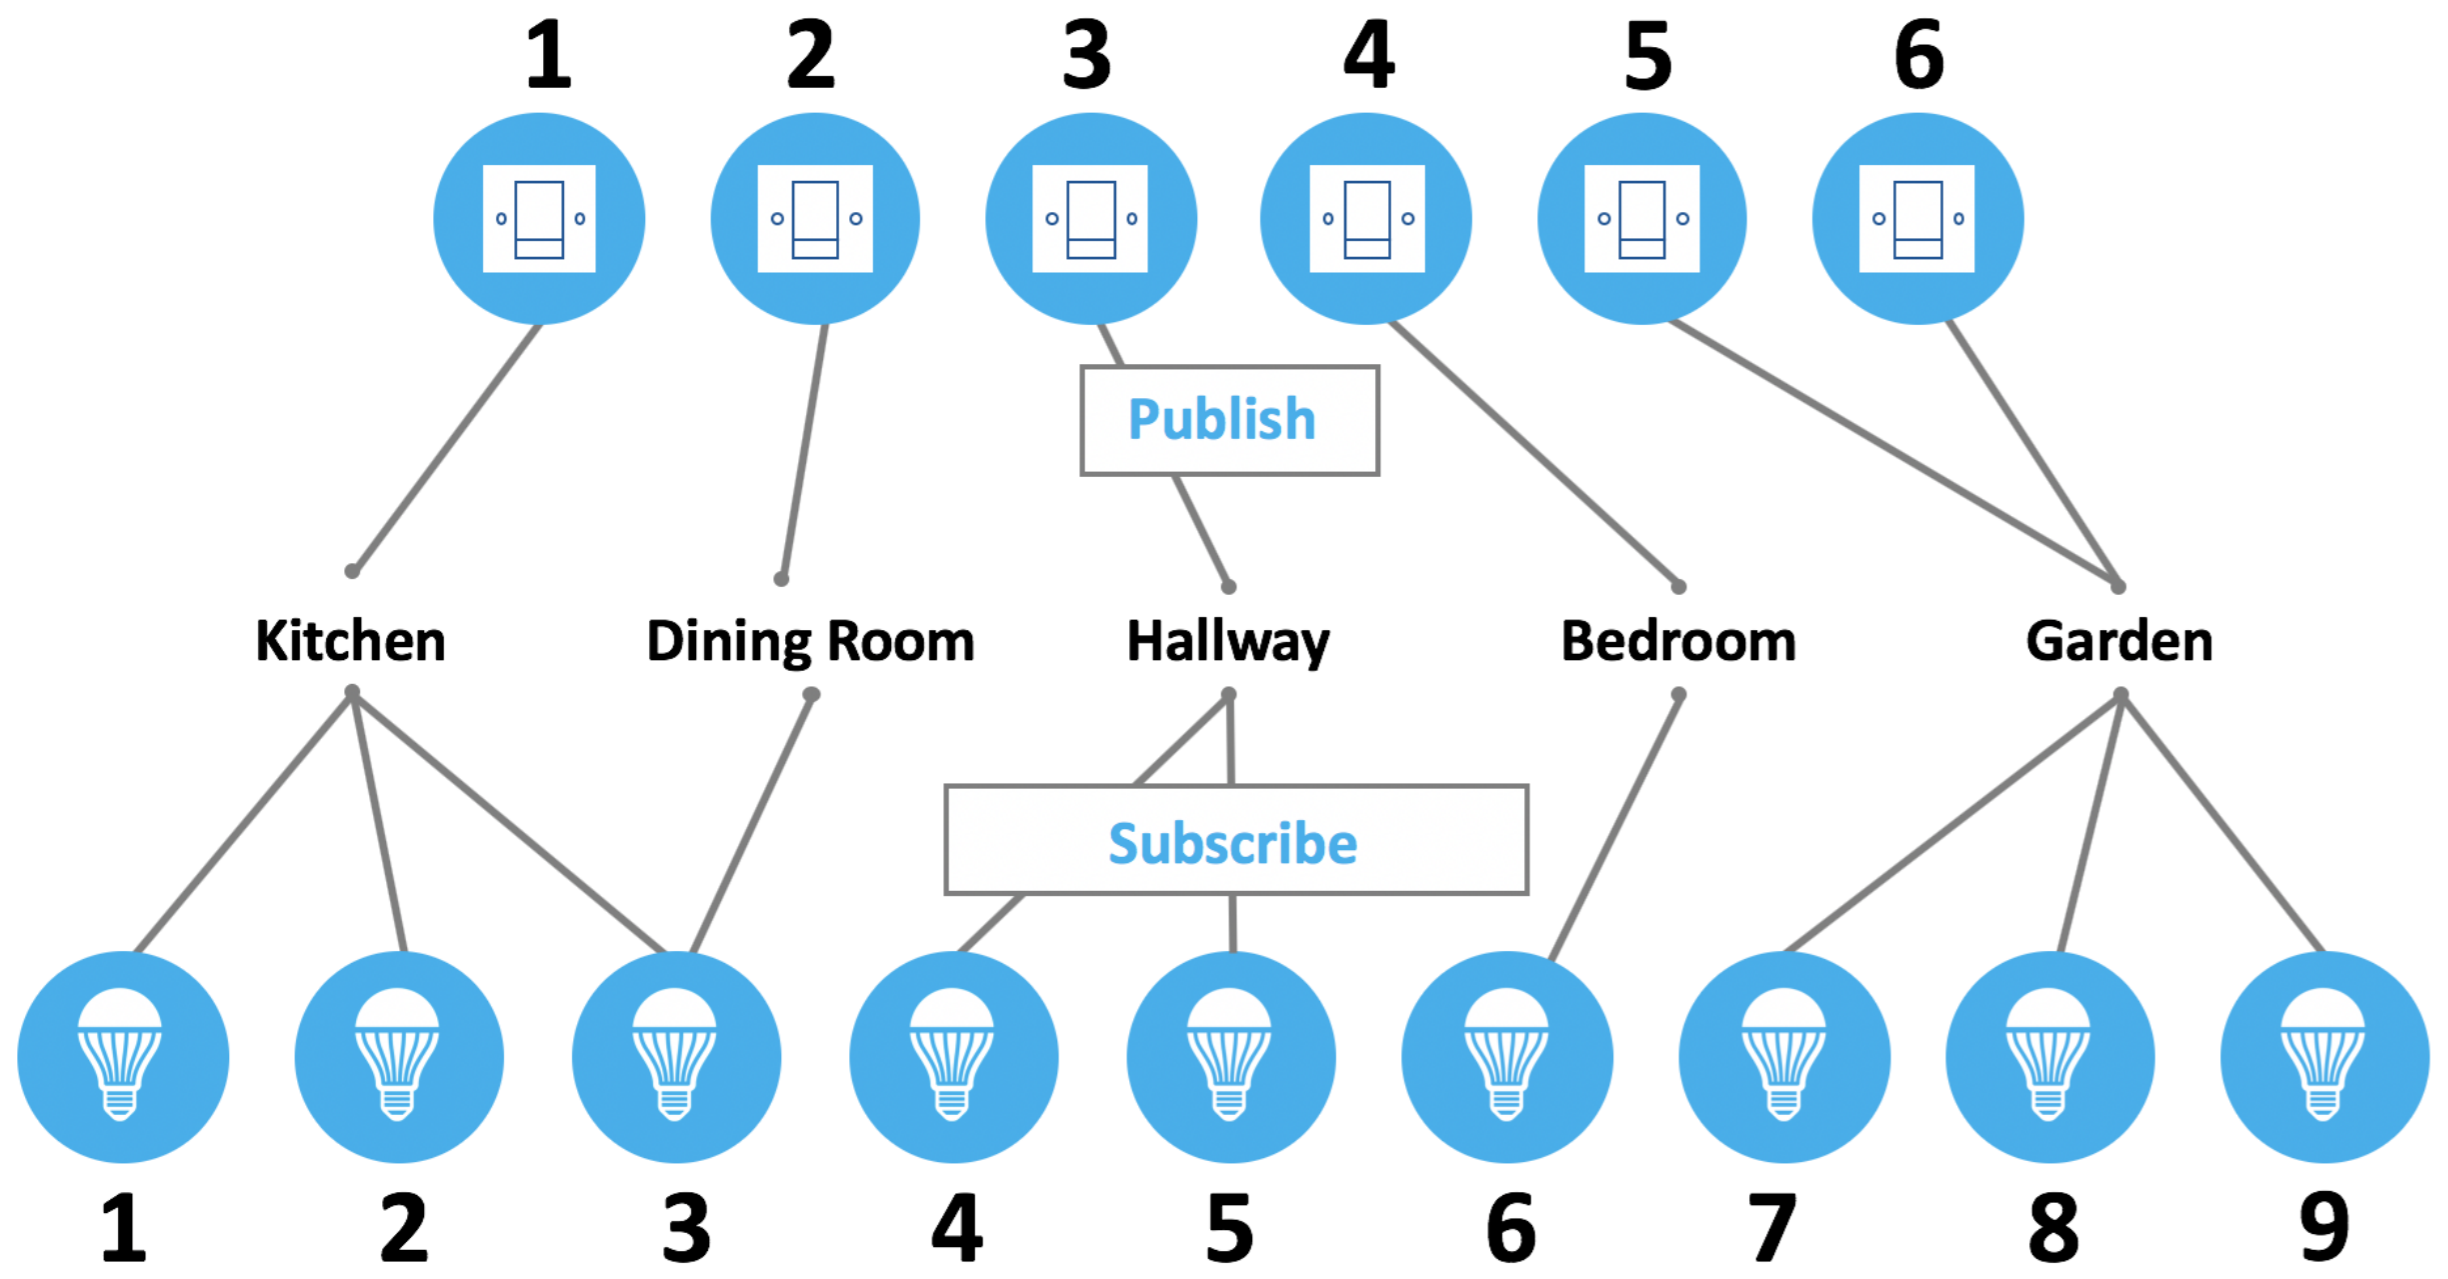
\includegraphics[width = \textwidth]{images/Publish_Subscribe_BLE.png}
    \caption{Esempio Publish-Subscribe}
    \label{fig:publish_subscribe_ble}
\end{figure}

\noindent Ogni messaggio viene inviato da un singolo unicast address ed identificato utilizzando un numero di sequenza univoco per facilitare il rilevamento e fronteggiare i possibili attacchi che prediligono la riproduzione di un messaggio.

\subsubsection{Managed Flooding}
\label{subsub:managed_flooding}
La comunicazione all'interno di una rete Mesh avviene tramite un meccanismo di flooding che prende il nome di \textit{Managed Flooding}. Tale tecnica utilizza i canali advertising per trasmettere messaggi in modo che gli altri nodi possano riceverli ed eventualmente ritrasmetterli, estendendo così la portata del messaggio originario. 
Senza una corretta gestione, il meccanismo di flooding, il quale prevede che ogni nodo debba ritrasmettere i messaggi ricevuti finché non viene raggiunto il nodo di destinazione, ridurrebbe gravemente la scalabilità, la robustezza della rete. %Un aspetto da non sottovalutare utilizzando un meccanismo di flooding è la possibilità di intasare la rete con messaggi superflui.
A tal proposito, il meccanismo adottato per le operazioni di routing all'interno di una rete Bluetooth Meesh prevede dei metodi per limitare il processo di inoltro, come: \textit{network message cache} e \textit{time to live}. In più tale standard consente di definire quali nodi debbano svolgere il ruolo di \textit{relay node}.\\
Il metodo network message cache è progettato per impedire ai dispositivi di inoltrare più volte il medesimo messaggio e, per tenerne traccia dei messaggi che sono stati già inviati, ogni messaggio ricevuto viene memorizzato in cache andando a creare una sorta di lista. In tal modo, ogni volta che viene ricevuto un messaggio, viene confrontato con questo elenco e se già presente il lista il messaggio viene ignorato, altrimenti si procede ad inoltrarlo e aggiungerlo alla lista. Operando in questo modo, con il crescere dei messaggi gestiti dal nodo, si potrebbe giungere ad avere un elenco infinito, difatti per evitare ciò, il numero di messaggi memorizzati in cache è limitato e può essere impostato tramite un apposito parametro in fase di configurazione del nodo.\\
Time to live (TTL) è un valore presente all'interno di ogni messaggio e limita il numero di volte che esso può essere inoltrato all'interno della rete. Ogni qualvolta che un messaggio viene ricevuto e poi inoltrato (fino ad un massimo di 126 volte), il valore TTL viene decrementato di 1. Nel momento in cui tale campo assume valore 0, il messaggio non potrà essere inoltrato, quindi verrà scartato.\\
Quindi, un relay node procederà ad inoltrare un messaggio solo se non è presente in cache e solo se il suo TTL è maggiore di 1.

\subsubsection{Modelli}
\label{subsub:modelli}
Il \textit{modello} implementa e definisce le funzionalità di base di un determinato nodo, ovvero provvede a definire gli stati, i messaggi che agiscono su di essi e qualsiasi comportamento associato a seguito di una transazione.\\
Un nodo può contenere molteplici modelli, e ognuno di essi determina le funzionalità dell'elemento cui si riferisce.\\
Tutte le comunicazioni all'interno di una rete Bluetooth sono eseguite per mezzo di messaggi i quali sono definiti come parte della specifica di un modello. Lo standard prevede tre categorie di modelli: client, server e control model.

\begin{itemize}
    \item un \textit{Server model} è composto da uno o più stati estesi tra uno o più elementi. Tale modello supporta appositi messaggi per operare sul comportamento relativo all'elemento o per comunicare il suo valore.
    
    \item un \textit{Client model} definisce un insieme di messaggi che il client usa per richiedere, modificare o utilizzare gli stati del server corrispondente, così come definito dal server model adottato. Il client model non ha stati.
    
    \item un \textit{Control model} può contenere sia le funzionalità di un client model sia le funzionalità di un server model per comunicare rispettivamente con altri server model o con altri client model.
\end{itemize}
Un singolo dispositivo può contenere anche tutti e tre i modelli appena descritti. 
Un modello, per includere funzionalità addizionali che gli consentono di gestire determinati comportamenti, deve essere obbligatoriamente esteso, anche perché tali modelli risultano immutabili, vale a dire che non è permesso modificare un modello aggiungendo o rimuovendo un comportamento.
Un modello che non estende altri modelli è chiamato \textit{root model}.\\
L'implementazione delle funzionalità dei nodi avviene attraverso i modelli, che possono essere divisi in SIG Model e Vendor Model, rispettivamente definiti da Bluetooth SIG e dai fornitori dei dispositivi o dagli utenti. In entrambi i casi, i modelli risultano identificabili attraverso un identificativo univoco di 16 bit per i modelli SIG e 32 bit per i modelli Vendor.

\subsubsection{Features}
\label{subsub:features}
Tutti i nodi hanno l'abilità di trasmettere e ricevere i messaggi. Tuttavia, le funzionalità di un nodo sono determinate dalle caratteristiche che esso supporta. I nodi possono supportare nessuna, una o più caratteristiche addizionali, abilitate o disattivate in qualsiasi momento:
\begin{itemize}
    \item \textit{Relay} feature: l'abilità di ritrasmettere quei messaggi inviati in broadcast dagli altri nodi. 
    Ciò consente di estendere la portata di ogni singola messaggio e fare in modo che possa attraversare l'intera rete con lo scopo di raggiungere anche tutti quei nodi non direttamente connessi al mittente. Con l'introduzione di questa caratteristica si ha la possibilità di creare una rete di grosse dimensioni.\\ % Managed Flooding
    Un nodo che supporta ed ha attiva tale funzionalità è definito come \textit{Relay node}.\\
    Il Relay node si preoccupa di inoltrare solo quei messaggi appartenenti alla propria sottorete. Nel caso di segmentazione del messaggio, il nodo provvederà ad inoltrare ogni singolo segmento una volta ricevuto, anziché attendere il messaggio completo.
    
    \item \textit{Proxy} feature: l'abilità di ricevere e ritrasmettere i messaggi tra GATT e advertising bearer. \\
    Tale caratteristica garantisce la retrocompatibilità per quei dispositivi BLE che non supportano Bluetooth mesh. In questo modo, un dispositivo BLE nativo come uno smartphone può anche comunicare con i dispositivi appartenenti ad una rete mesh. 
    In tale circostanza si ha un dispositivo connection-oriented con il nodo proxy e quest'ultimo tramite le operazioni messe a disposizione dallo standard BLE (operazioni GATT) è in grado di agire da intermediario e quindi consentire a questa tipologia di dispositivi ad interfacciarsi ed interagire con i nodi appartenenti alla rete mesh.\\
    Quindi, attraverso la seguente funzionalità il nodo è in grado di eseguire una traduzione tra le PDU proxy e le PDU mesh. Il nodo che supporta ed ha attiva tale funzionalità è conosciuto \textit{Proxy node}.
    
    \item \textit{Low Power} feature: la capacità di operare all'interno di una rete mesh con un duty cycle significativamente ridotto. La sua presenza all'interno di una rete mesh è resa possibile solo in combinazione con un nodo che supporta la relazione ``Friendship''.\\
    Un nodo che supporta tale funzionalità ed ha attiva un'amicizia con un Friend node è definito \textit{Low Power node} e tramite un meccanismo di polling ottiene informazioni dal suo Friend node.
    
    \item \textit{Friend} feature: la capacità di supportare un Low Power node, difatti è responsabile della memorizzazione dei messaggi destinati ai suoi nodi ``amici'' e dell'inoltro di messaggi generati da questi nodi all'interno della rete. A tal proposito ogni nodo amico dovrebbe essere anche un nodo relay.\\
    Un nodo che supporta ed ha attiva tale funzionalità, ed inoltre ha un'amicizia con un Low Power node è definito \textit{Friend node}. L'aver abilitato la funzionalità Friend può comportare un maggior consumo energetico, a tal proposito questi nodi risultano, molto spesso, essere alimentati tramite la rete elettrica.
\end{itemize}

\paragraph{Friendship}
Friendship è una speciale relazione tra un \textit{Low Power node} e un \textit{Fiend node} che consente la presenza del primo all'interno di una rete mesh. Tale relazione consente al nodo con poche risorse energetiche di limitare la quantità di tempo in cui debba essere in ascolto e soprattutto consente di evitare la perdita di messaggi ad esso destinati. Affinché sia attuabile tale relazione questi due tipi di nodi devono essere adiacenti, ovvero trovarsi ad un singolo hop di distanza e nella medesima sottorete.\\

\noindent Il nodo Low Power solitamente ha un'alimentazione limitata (a batteria) e provvede a risparmiare energia mantenendo la radio spenta il più possibile, garantendo così un ridotto duty cycle. Il nodo periodicamente si sveglia per eseguire delle interazioni con il nodo amico per poi tornare nuovamente in sleep mode. Le interazioni prevedono il polling dal nodo Friend per recuperare i messaggi ad esso destinati e se necessario procede con l'invio di messaggi ai nodi della rete.\\
Il nodo Low Power necessita di un nodo Friend per poter stabilire tale relazione, infatti la procedura che consente di giungere in questo stato è avviata proprio dal nodo Low Power. Una volta stabilita la relazione, il nodo Friend esegue una serie di azioni che aiutano a ridurre il consumo di energia al nodo a bassa potenza permettendogli di programmare la frequenza appropriata per l'impiego della propria radio e quindi l'operazione di polling per verificare la presenza di nuovi messaggi ad esso destinati.\\
Il nodo Friend utilizza una Friend Queue per memorizzare tutti i messaggi in arrivo indirizzati ai propri nodi amici e provvede a recapitarli quando richiesto da tali nodi. Inoltre, garantisce anche supporto in merito agli aggiornamenti relativi alla sicurezza per i suoi nodi amici.\\
Una volta che la relazione è stabilita tra i due nodi, essi sono considerati ``friends''. Un nodo Friend può essere amico con più nodi Low Power, mentre un nodo Low Power può avere un unico Friend node.\\

\noindent Solitamente i nodi Low Power sono dei semplici sensori che si occupano di inviare periodicamente la lettura del valore acquisito in broadcast nella rete e non sono soggetti alla ricezione di molti messaggi. Gli unici messaggi che solitamente ricevono riguardano la configurazione di determinate soglie, come ad esempio l'intervallo di tempo con cui il nodo deve inviare i dati acquisiti.

\paragraph{Mesh Gateway}
Un mesh gateway è quel nodo in grado di tradurre i messaggi tra una rete mesh e una tecnologia non Bluetooth.

\section{Provisioning}
\label{sec:provisioning}
% %.4.2 Provisioning behaviour
% https://www.bluetooth.com/blog/provisioning-a-bluetooth-mesh-network-part-1/
% https://www.bluetooth.com/blog/provisioning-a-bluetooth-mesh-network-part-2/
Il processo di provisioning è uno dei concetti più importanti in BLE Mesh. Consente, mediante uno scambio di informazioni tra un unprovisioned device ed un provisioner di aggiungere il dispositivo all'interno di una rete mesh. Il processo è gestito da un provisioner, in genere uno smartphone o un altro dispositivo di elaborazione mobile in grado di eseguire un'applicazione di provisioning.\\
La specifica Bluetooth mesh definisce il protocollo di provisioning ed il suo funzionamento. Per eseguire tale procedura sono state definite apposite PDU, necessarie per comunicare tra un provisioner ed un nuovo dispositivo che desidera entrare a far parte di una rete mesh.

\begin{figure}[!ht]
    \centering
    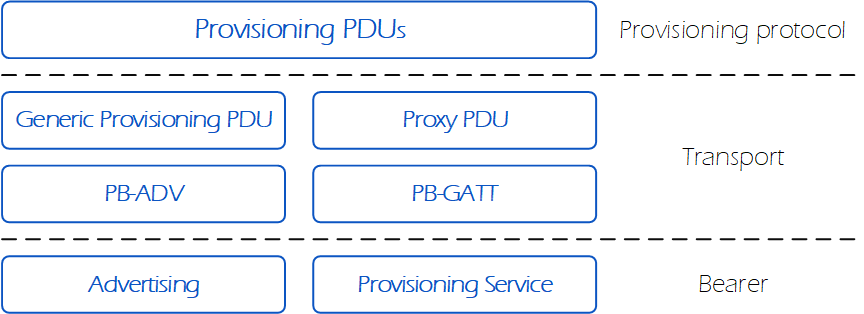
\includegraphics[width = \textwidth]{images/Provisioning_architecture.png}
    \caption{Provisioning protocol stack}
    \label{fig:provisioning_stack}
\end{figure}

\begin{itemize}
    \item il \textit{Provisioning Bearer} layer consente il trasporto di apposite PDU tra il provisioner e un unprovisioned device, definendo due tipologie di Bearer:
    \begin{itemize}
        \item \textit{PB-ADV}: una tecnica di provisioning bearer utilizzato per eseguire la procedura di provisioning di un dispositivo sfruttando i canali advertising. Il PB-ADV bearer è utilizzato per trasmettere Generic Provisioning PDU.\\
        Un dispositivo che supporta PB-ADV dovrebbe eseguire la scansione passiva con un duty cycle vicino al 100\% per evitare di perdere qualsiasi Generic Provisioning PDU in arrivo.
        
        \item \textit{PB-GATT}: un provisioning bearer che consente ad un dispositivo che non supporta PB-ADV di comunicare indirettamente con i nodi di una rete mesh incapsulando i Provisioning PDU all'interno di proxy PDU avvalendosi di un proxy node. Il protocollo proxy consente ai nodi di inviare e ricevere network PDU, mesh beacon, messaggi di configurazione proxy e provisioning PDU avvalendosi di una connessione orientata eseguita utilizzando lo standard BLE (canali Data).
    \end{itemize}
    
    \item il \textit{Provisioning Protocol} definisce i requisiti in merito alle PDU, comportamento e sicurezza. Sono state definite 10 provisioning PDU: Provisioning Invite, Provisioning Capabilities, Provisioning State, Provisioning Public Key, Provisioning Input Complete, Provisioning Confirmation, Provisioning Random, Provisioning Data, Provisioning Complete, Provisioning Failed.
\end{itemize}

\noindent La procedura di provisioning deve svolgere due importanti compiti di alto livello:
\begin{enumerate}
    \item autenticare l'unprovisioned device. L'autenticazione viene eseguita per assicurare che il dispositivo con cui interagisce il provisioner sia il dispositivo che l'utente vuole far subentrare nella rete mesh.
    
    \item creare un collegamento sicuro tra i due dispositivi e procedere con la condivisione delle informazioni, tra cui la chiave di rete e l'indirizzo unicast per ogni elemento presente nel nodo.
\end{enumerate}

\subsection{Provisioning Procedure}
La procedura di provisioning prevede cinque fasi: Beaconing, Invitation, Exchange public keys, Authentication e Distribution of provisioning data.

\subsubsection{Beaconing}
Un dispositivo che vuole subentrare all'interno di una rete mesh e supporta \textit{PB-ADV}, pubblicizza la propria presenza inviando in broadcast di appositi pacchetti (Unprovisioned Device Beacon) sui canali di advertising.\\
Quando viene usato PB-GATT da un unprovisioned device, la procedura di provisioning e le interazione con il provisioner sono supportate da un servizio GATT chiamato Mesh Provisioning Service. Nella fase di Beaconing il dispositivo che vuole entrare a far parte della rete trasmette in broadcast pacchetti pubblicitari contenenti l'UUID del Mesh Provisioning Service e viene individuato dal provisioner tramite la procedura di scansione dello standard BLE. 
Con tale fase, il dispositivo indica al provisioner la disponibilità ad avviare il processo di provisoning.

\subsubsection{Invitation}
Dopo la fase di Beaconing, il provisioner e l'unprovisioned device stabiliscono una provisioning bearer, vale a dire che il provisioner individua i beacon inviati sui canali advertising e provvederà ad inviare un Provisioning Invite PDU al nuovo dispositivo, il quale si appresterà a rispondere tramite un Provisioning Capabilities PDU.\\
Il Provisioning Invite PDU include un campo Attention Duration che indica per quanto tempo l'elemento primario del unprovisioned device deve attirare l'attenzione dell'utente usando l'Attention Timer, una qualche forma di indicazione visiva.\\
Il Provisioning Capabilities PDU include:
\begin{itemize}
    \item il numero di elementi supportati dal dispositivo.
    \item l'insieme degli algoritmi di sicurezza supportati.
    \item la disponibilità della sua public key utilizzando il metodo Out-of-Band (OOB).
    \item la capacità del dispositivo di fornire un valore in output all'utente.
    \item la capacità di un dispositivo di ricevere in input un valore dall'utente.
\end{itemize}
\noindent La seguente fase ha l'obiettivo di fornire al provisioner le informazioni in merito alle capacità supportate dal device e in base a ciò verrà decisa la modalità utilizzata per eseguire la procedura di provisoning.

\begin{figure}[!ht]
    \centering
    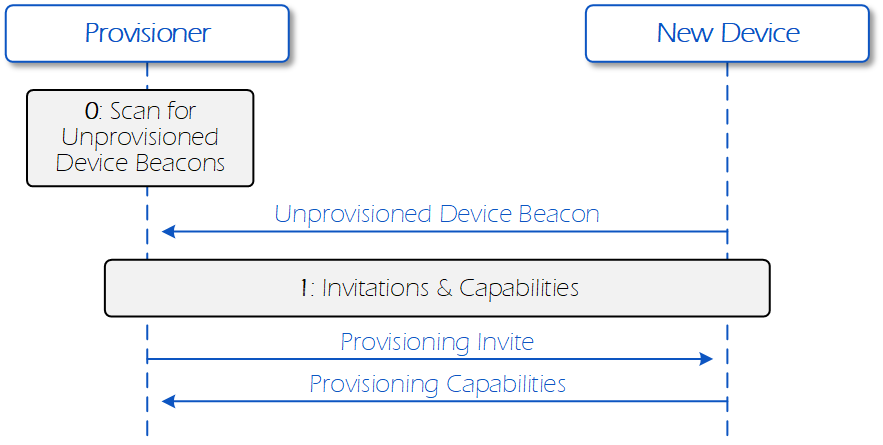
\includegraphics[width = \textwidth]{images/Provisioning_Invitation.png}
    \caption{Provisioning Invitation}
    \label{fig:provisioning_invitation}
\end{figure}

\subsubsection{Exchange public keys}
% https://www.bluetooth.com/blog/provisioning-a-bluetooth-mesh-network-part-1/
Questa fase riguarda un aspetto di sicurezza e prevede la combinazione di due tecniche di crittografia per scambiare delle informazioni in modo sicuro: cifratura simmetrica (crittografia a chiave segreta) e cifratura asimmetrica (crittografia a chiave pubblica).

\begin{itemize}
    \item la \textit{cifratura Simmetrica} utilizza la stessa chiave segreta sia per la cifratura che per la decifratura. Nel momento che mittente e destinatario conoscono la chiave segreta, possono decrittografare tutti i messaggi crittografati con tale chiave. La problematica di tale procedura riguarda lo scambio in totale sicurezza della chiave segrete su un collegamento e impedire che cadano in mani sbagliate.

    \item la \textit{cifratura asimmetrica} utilizza due chiavi correlate proprio per risolvere il problema sopra citato: chiave pubblica e chiave privata. Qualsiasi messaggio viene cifrato utilizzando la chiave pubblica e può essere decifrato solo applicando lo stesso algoritmo e la chiave privata corrispondente. Tuttavia, questa tecnica è più lenta della precedente e richiede molta più potenza di elaborazione per crittografare e decrittografare il contenuto dei messaggi.
\end{itemize}

\noindent Poiché la tecnica asimmetrica risulta essere computazionalmente costosa per i dispositivi coinvolti e poiché la tecnica simmetrica non garantisce uno scambio di chiavi in modo sicuro, Bluetooth Mesh utilizza una combinazione di metodi simmetrici e asimmetrici per fronteggiare tale problematica.\\
Tale combinazione prevede l'utilizzo dell'Elliptic-curve Diffie-Hellman (ECDH), un protocollo che consente a due parti, ognuna con una coppia di chiavi elliptic curve pubblica-privata, di stabilire un segreto condiviso su un canale non sicuro. Lo scopo di tale algoritmo in nella fase di provisioning riguarda la creazione di un collegamento sicuro tra il provisioner e l'unprovisioned device. Prevede l'uso di chiavi pubbliche e private per distribuire una chiave simmetrica che i due dispositivi possono utilizzare per crittografare e decrittografare i successivi messaggi. Quindi ogni messaggio trasmesso in una rete mesh verrà crittografato utilizzando la crittografia AES-128.\\

\noindent Nella fase di Exchange public keys a seconda delle capacità del dispositivo, scoperte nella fase precedente, il provisioner sceglie la modalità con cui scambiare le chiavi pubbliche ECDH. Lo scambio può avvenire tramite un normale collegamento Bluetooth o tramite la tecnologia OOB.
Dopo aver scelto la metodologia, informa il device tramite l'invio di un Provisioning Start PDU contenente l'approccio da adottare.\\

\noindent Se lo scambio di chiavi pubbliche non è possibile tramite la tecnologia OOB, esso avverrà direttamente tramite un collegamento Bluetooth. Per ogni scambio, una nuova coppia di chiavi deve essere generata sia dal provisioner sia dall'unprovisioned device.

\begin{figure}[!ht]
    \centering
    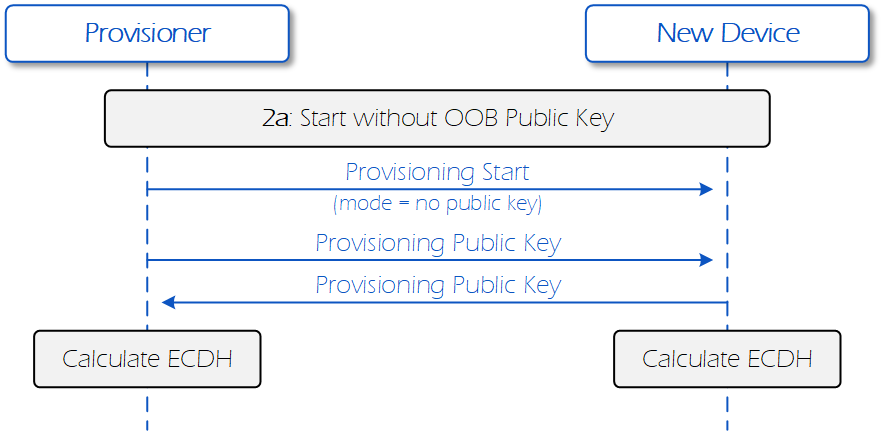
\includegraphics[width = \textwidth]{images/Provisioning_public_key_exchange_a.png}
    \caption{Public Key Exchange quando la public key dell'unprovisioned device è sconosciuta}
    \label{fig:provisioning_public_key_a}
\end{figure}

\noindent Altrimenti, se è possibile scambiare la chiave pubblica attraverso il meccanismo OOB, una nuova coppia di chiavi verrà generata solo dal Provisioner e la chiave pubblica relativa verrà trasmessa al dispositivo, il quale sarà in grado di leggere una chiave pubblica statica utilizzando il meccanismo OOB.

\begin{figure}[!ht]
    \centering
    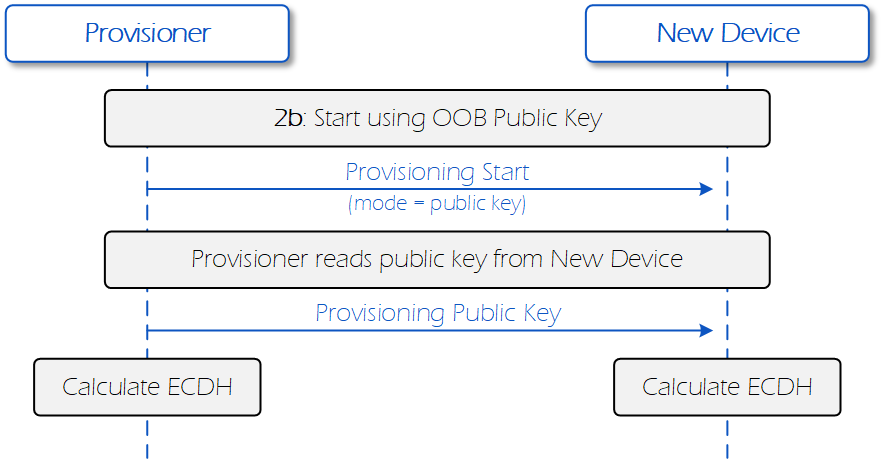
\includegraphics[width = \textwidth]{images/Provisioning_public_key_exchange_b.png}
    \caption{Public Key Exchange tramite il metodo OOB}
    \label{fig:provisioning_public_key_b}
\end{figure}

\noindent I dispositivi coinvolti dovranno verificare se la chiave pubblica ottenuta risulti valida. Se la chiave non è valida il processo di provisioning fallisce. Dopo che la chiave pubblica è nota ed è stata convalidata, ogni dispositivo calcola una chiave simmetrica, nota come ECDHSecret, utilizzando la propria chiave privata e la chiave pubblica del dispositivo peer. Questa chiave verrà utilizzata per proteggere la comunicazione tra i dispositiva da questo punto in avanti.\\
Solo dopo aver calcolato ECDHSecret, i due dispositivi dovranno eliminare la coppia di chiavi pubblica-privata generate in precedenza.

\subsubsection{Authentication}
% https://www.bluetooth.com/blog/provisioning-a-bluetooth-mesh-network-part-2/
Il prossimo step, prevede l'autenticazione del dispositivo. In questo step, il provisioner utilizzerà il metodo di autenticazione selezionato (in base alle capacità del dispositivo) e comunicato al dispositivo all'interno del Provisioning Start PDU. Esistono quattro approcci disponibili: Output OOB, Input OOB, Static OOB e No OOB. Solitamente richiede un'azione da parte dell'utente, il quale dovrà interagire sia con il dispositivo provisioner sia con l'unprovisioned device.

\paragraph{Output OOB}
Se si seleziona il metodo Output OOB, l'unprovisioned device genera un numero casuale e lo mostra all'utente in base alle sue capacità (se è una lampadina potrebbe lampeggiare un determinato numero di volte). Tale numero dovrà essere inserito dall'utente sul dispositivo in grado di supportare un'applicazione di provisioning e tal modo il provisioner potrà autenticare il dispositivo. \\
Il processo di autenticazione continua con l'operazione di \textit{check confirmation value}.

\begin{figure}[!ht]
    \centering
    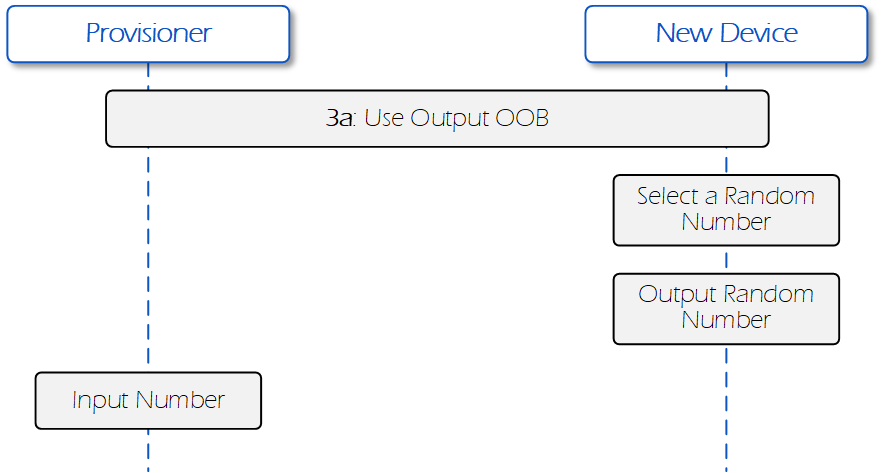
\includegraphics[width = \textwidth]{images/Provisioning_OOB_output.png}
    \caption{Autenticazione con Output OOB}
    \label{fig:provisioning_output_OOB}
\end{figure}

\paragraph{Input OOB}
Il seguente metodo è simile al precedente, ma prevede un'inversione dei ruoli. Il provisioner genera e mostra un numero casuale, dopodiché richiede all'utente di inserirlo nell'unprovisioned device mediante un'azione appropriata e supportata da quest'ultimo.\\
Dopo aver completato l'autenticazione, il dispositivo provvede a comunicare al provisioner, tramite un Provisioning Input Complete PDU, l'avvenuto inserimento del numero casuale. Il processo continua con il \textit{check confirmation value}.

\begin{figure}[!ht]
    \centering
    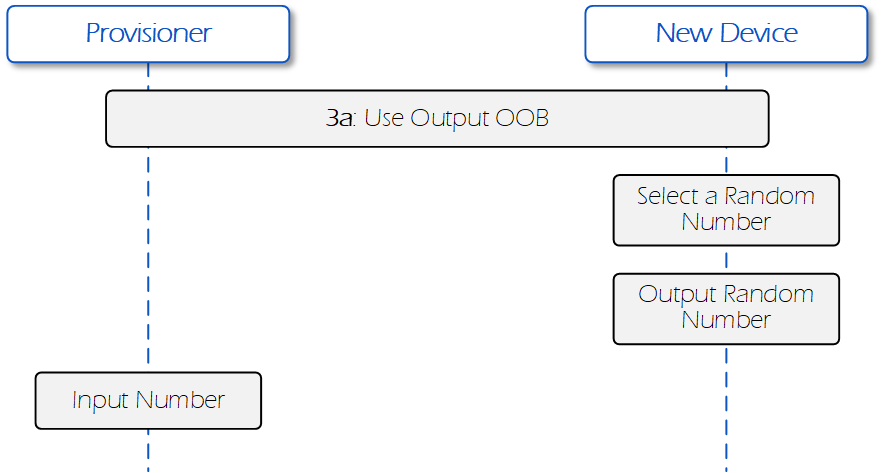
\includegraphics[width = \textwidth]{images/Provisioning_OOB_output.png}
    \caption{Autenticazione con Input OOB}
    \label{fig:provisioning_input_OOB}
\end{figure}

\paragraph{Static OOB o No OOB}
Nel caso in cui non è possibile scegliere i due metodi sopra menzionati, si ricorre all'autenticazione Static OOB o all'autenticazione No OOB.
In ogni caso, ognuno dei due dispositivi genera un numero e si procede con l'operazione di \textit{check confirmation value}, senza la necessità dell'interazione da parte dell'utente. \\
Nel caso della tecnica Static OOB si ricorre all'uso di un valore statico per autenticare il dispositivo. Nel caso della tecnica No OOB si utilizza il valore 0 nel campo relativo allo Static OOB. Utilizzare quest'ultima tecnica è come non autenticare il dispositivo.

\paragraph{Check confirmation value}
L'operazione prevede in primo luogo di calcolare in modo indipendente, per ciascun device, un valore di conferma, conosciuti come \textit{ConfirmationProvisioner} e \textit{ConfirmationDevice} e dopodiché la validazione del valore da parte dell'altro dispositivo. La funzione di generazione del valore di conferma richiede otto parametri i cui valori provengono dalle fasi del processo di provisioning.

\begin{figure}[!ht]
    \centering
    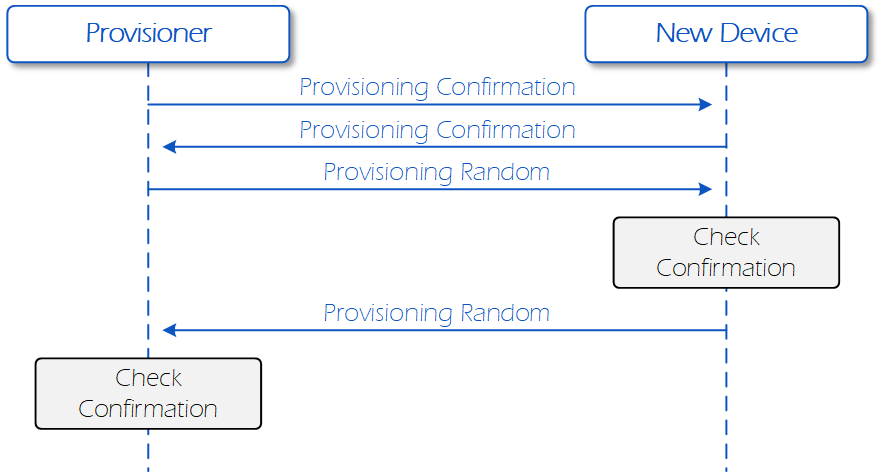
\includegraphics[width = \textwidth]{images/Provisioning_confirmation_value_check.png}
    \caption{Confirmation value check}
    \label{fig:provisioning_confirmation_value_check}
\end{figure}

\noindent Quando i valori di conferma risultano generati, i due dispositivi si scambiano tale informazione e ciascuno controlla l'integrità del valore ricevuto.\\
Il processo di conferma inizia con il provisioner che invia un valore casuale (RandomProvisioner) al peer e quest'ultimo tramite tale valore ricalcola il valore di conferma e lo verifica con il ConfirmationProvisioner. Se non c'è corrispondenza tra i due valori, il processo di provisioning viene interrotto. Altrimenti, il device procede con l'invio di un numero casuale (RandomDevice) al provisioner.\\
Il provisoner, a questo punto, usa lo stesso processo per ricalcolare il valore di conferma e lo verifica confrontandolo con il valore ricevuto in precedenza. Se il valore calcolato non corrisponde al ConfirmationDevice, il processo sarà interrotto. Altrimenti, vorrà dire che l'autenticazione avrà esito positivo e il dispositivo potrà diventare un membro della rete mesh.

\subsubsection{Distribution of provisioning data}
Una volta completata la fase di autenticazione si procede alla fase più importante della procedura: derivazione e distribuzione dei provisioning data. Il provisioner è responsabile della generazione di tali dati, che consistono in una serie di elementi, tra cui la Network Key, la Device Key, un parametro di sicurezza conosciuto come IV index e l'Unicast Address che viene assegnato al dispositivo da parte del provisioner.\\
Per distribuire i ``provisoning data'' in modo sicuro, il provisoner utilizza l'algoritmo AES-CCM per crittografare tali dati con una SessionKey, che entrambi i dispositivi dovranno calcolare. La session Key verrà derivata da ciascun dispositivo usando la propria chiave privata e la chiave pubblica ricevuta dall'altro dispositivo. Una volta calcolata, il povisioner si appresta a cifrare ed inviare la Provisioning Data PDU. 
Dopo aver ricevuto i dati dal Provisioner, il dispositivo dovrà decriptarli (usando la Session Kye) e autenticarli. A termine di queste due operazioni, provvederà ad impostare i vari parametri (tra cui la network key e l'unicast address). Al completamento della procedura che assegna l'indirizzo unicast, il dispositivo risponderà al Provisioner con una  Provisioning Complete PDU per confermare l'esito positivo della procedura.

\begin{figure}[!ht]
    \centering
    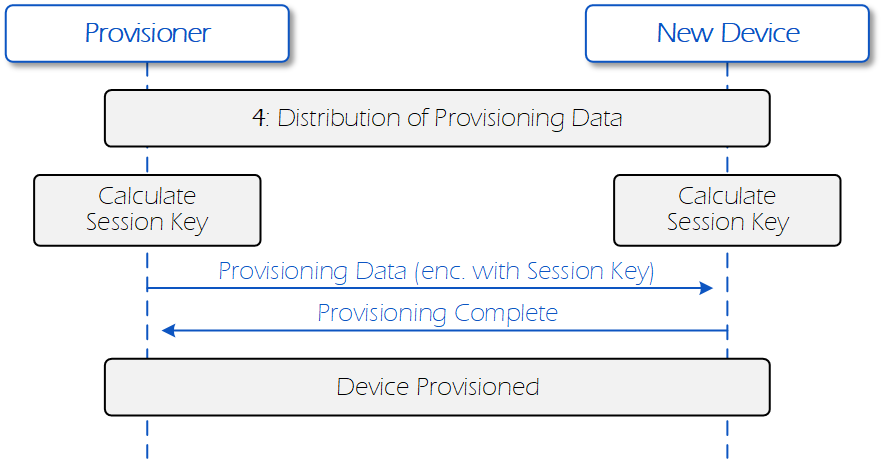
\includegraphics[width = \textwidth]{images/Provisioning_distribution_data.png}
    \caption{Distribution of provisioning data}
    \label{fig:provisioning_distribution_data}
\end{figure}

Con quest'ultimo passaggio, che sancisce la terminazione della procedura di provisioning, l'unprovisioned device diventerà un membro della rete mesh e potrà essere definito \textit{nodo}.

\section{Security}
% https://www.novelbits.io/bluetooth-mesh-tutorial-part-3/
Un aspetto molto importante in Bluetooth Mesh riguarda la sicurezza, rispetto a BLE in cui la sicurezza è facoltativa e la scelta di includerla o meno viene lasciata allo sviluppatore, in Bluetooth mesh è obbligatoria.\\
Lo standard Bluetooth Mesh prevede che tutti i messaggi all'interno di una rete mesh devono essere crittografati e autenticati tramite apposite chiavi di sicurezza, gestite in modo indipendente dall'upper transport layer e dal network layer. \\
Conservando le due chiavi in modo distinto consente di poter distinguere messaggi con contenuti sensibili (controllo dell'accesso ad un edificio) da messaggi non sensibili (luci di un'abitazione) e consentendo così l'inoltro di un messaggio a qualsiasi nodo della rete (tramite la chiave di rete) senza dover conoscere la chiave di applicazione (non avendo così la possibilità di modificare o comprendere i dati del livello di applicazione).\\

\noindent Il modello di sicurezza definisce due principali chiavi di sicurezza: la chiave del livello di rete (NetKey) e la chiave del livello applicativo (AppKey). In più, è definita un tipo speciale di AppKey conosciuta come DeviceKey (DevKey).

\begin{itemize}
    \item la \textit{Network Key} consente di rendere sicura la comunicazione a livello di rete ed è condivisa da tutti i nodi della rete o da tutti i nodi appartenenti ad una particolare sottorete. Il possesso di una determinata chiave di rete è ciò che rende un nodo, partecipe ad una rete mesh o sottorete e quindi gli consente di decriptare le comunicazioni inerenti. Dalla NetKey sono derivate altre due chiavi: la network encryption key e la privacy key. \\
    I nodi in possessori di una NetKey sono in grado di decriptare e autenticare un messaggio, ovvero con tale chiave hanno la possibilità di accedere fino al contenuto del livello di rete, consentendo così l'inoltro di un messaggio ma nessuna decodifica dei dati applicativi.

    \item l'\textit{Application Key} consente di rendere sicura la comunicazione a livello Access ed è condivisa da un gruppo ristretto di nodi, normalmente quelli che partecipano ad una data funzionalità all'interno della mesh (mesh Application). Ad esempio, un AppKey legata all'illuminazione sarà condivisa solo tra interruttori e lampadine e non con un termostato o una sensore di movimento. Solitamente, un AppKey coinvolge tipi correlati di dispositivi. \\ 
    Un AppKey è usata per autenticare e decriptare i dati del livello di applicazione all'interno di una singola rete mesh, difatti la sua validità è confinata alla singola rete.
    
    \item la \textit{Device Key} è una chiave univoca appartenente ad ogni nodo ed è conosciuta solo da quest'ultimo e dal Provisioner. A tal proposito, viene utilizzata durante il processo di provisioning per creare una comunicazione sicura tra i due partecipanti (unprovisioned device e provisioner). Adoperando la DevKey è possibile distribuire in modo sicuro la NetKey e la AppKey.

\end{itemize}

\paragraph{Obfuscation}
Il modello di sicurezza adottato dal livello di rete usa un meccanismo di privacy, chiamato Obfuscation, che utilizza AES per crittografare l'indirizzo di origine, i numeri di sequenza e altre informazioni dell'header di un messaggio avvalendosi della privacy key. L'obbiettivo dell'offuscamento è rendere più difficile il processo di tracking.

\paragraph{Key identifiers}
Un nodo può avere più chiavi di rete e di applicazione. Utilizzando un key identifier è possibile identificare quale sottoinsieme di chiavi è usato per proteggere il messaggio. L'identificatore viene generato dalla chiave di rete o di applicazione usando un'apposita funzione di derivazione della chiave.

\subsubsection{Problemi}
Una della maggiori preoccupazioni con una rete mesh è che un possibile attaccante possa ottenere l'accesso alla rete servendosi di quei dispositivi che non fanno più parte della rete. Per proteggersi da questo tipo di attacco, lo standard Bluetotth mesh definisce una procedura per la rimozione di un nodo. Tale dispositivo verrà inserito in un'apposita lista (blacklist) e le chiavi vengono rigenerate. Tale procedura prevede quindi di distribuire nuove chiavi di rete, di applicazione e altri dati importanti per i vari nodi, ad eccezione di quelli messi in blacklist.\\
Un altro problema da fronteggiare riguarda i \textit{replay attack}. Un replay attack è quando uno o più messaggi sono memorizzati e riproposti successivamente da un dispositivo malizioso. Per fronteggiare questa tipologia di attacco lo standard addotta:
\begin{itemize}
    \item \textit{numeri di sequenza} (SEQ). Ogni elemento incrementa il numero di sequenza ogni volta che pubblica un messaggio. Un nodo che riceve un messaggio da un elemento che contiene un valore SEQ inferiore o uguale dell'ultimo messaggio valido, lo scarterà.
    
    \item IV index incrementale, un valore aggiuntivo che viene validato quando viene ricevuto un messaggio.
\end{itemize}

% https://www.nordicsemi.com/Software-and-tools/Development-Tools/nRF-Mesh